\begin{frame}{Le progrès de la science comme un processus discontinu}
\begin{block}{Rupture épistémologique}
Passage radical d'un paradigme\footnote{découverte scientifique universellement reconnue.} à un autre, dans la façon dont les scientifiques abordent un domaine donné.
\end{block}
\begin{itemize}
\small
\item \leftguillemet{} rupture entre observation et expérimentation \rightguillemet{} 
{\footnotesize(\cite{bachelard1934formation})}
\item \leftguillemet{} révolution scientifique \rightguillemet{} {\footnotesize(\cite{koyre1957closed})}
\item \leftguillemet{} changement de paradigme \rightguillemet{} {\footnotesize(\cite{kuhn1962structure})} 
\end{itemize} 
%Le nouveau paradigme est incompatible avec le précédent, p. ex. géo- \textit{vs.} héliocentrisme.
\begin{minipage}{5cm}
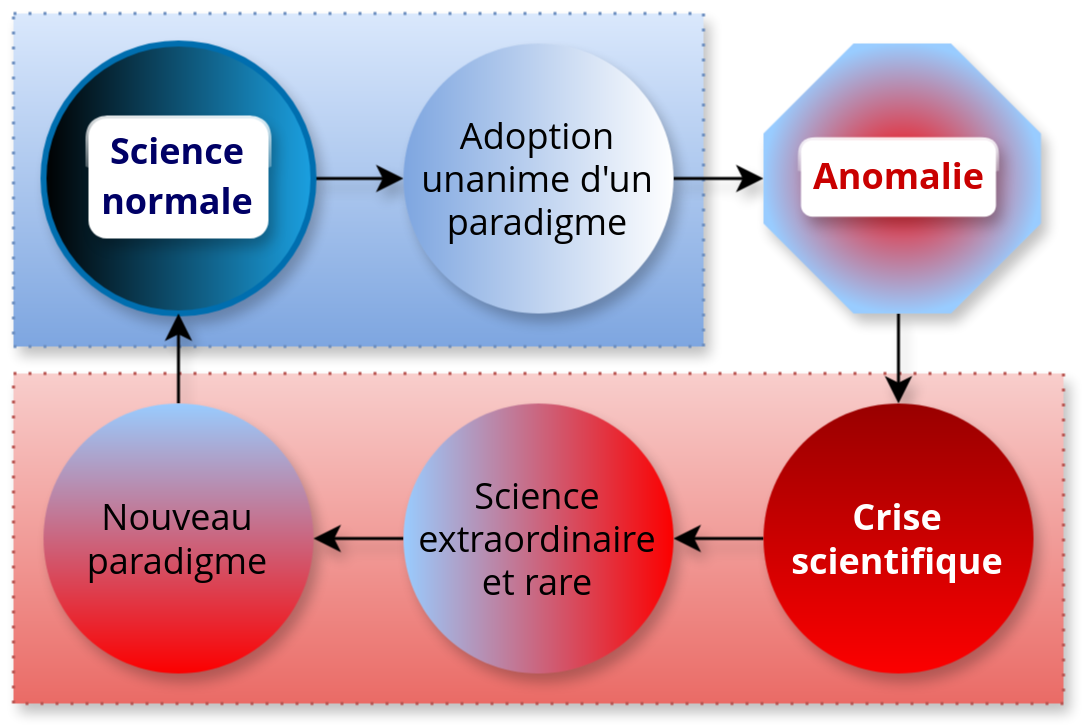
\includegraphics[height=3cm, width=4.5cm]{pic/changement_paradigme.png}
\end{minipage}%
\begin{minipage}{6cm}
{\normaltext Conception kuhnienne du progrès scientifique, adaptée de {\small\textcite{amiri}}}. \bigskip

 {\scriptsize Le nouveau paradigme est incompatible avec le précédent, p. ex. géo- \textit{vs.} héliocentrisme.}
\end{minipage}
%\begin{figure}
%    \centering
%    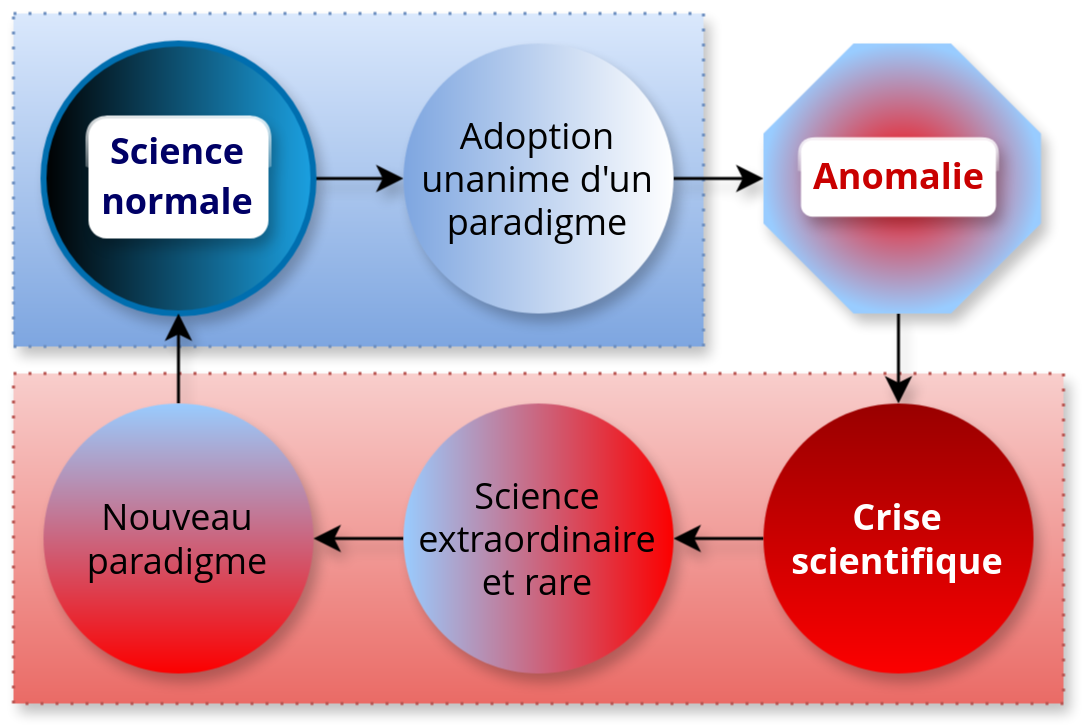
\includegraphics[width=65mm,scale=0.5]{pic/changement_paradigme.png}
%    \caption{Conception kuhnienne du progrès scientifique, adaptée de {\scriptsize\textcite{amiri}}.}
%    \label{fig:enter-label}
%\end{figure}
\end{frame}
